\subsection{Mechanik}

\begin{tabularx}{\columnwidth}{p{3cm}XX}
	Mech. Drehmoment \newline Torque& $\bm\tau = \bm r\times \bm F$\newline $\tau = |\bm r| |\bm F| sin\theta$ 
	& \vspace*{-1cm}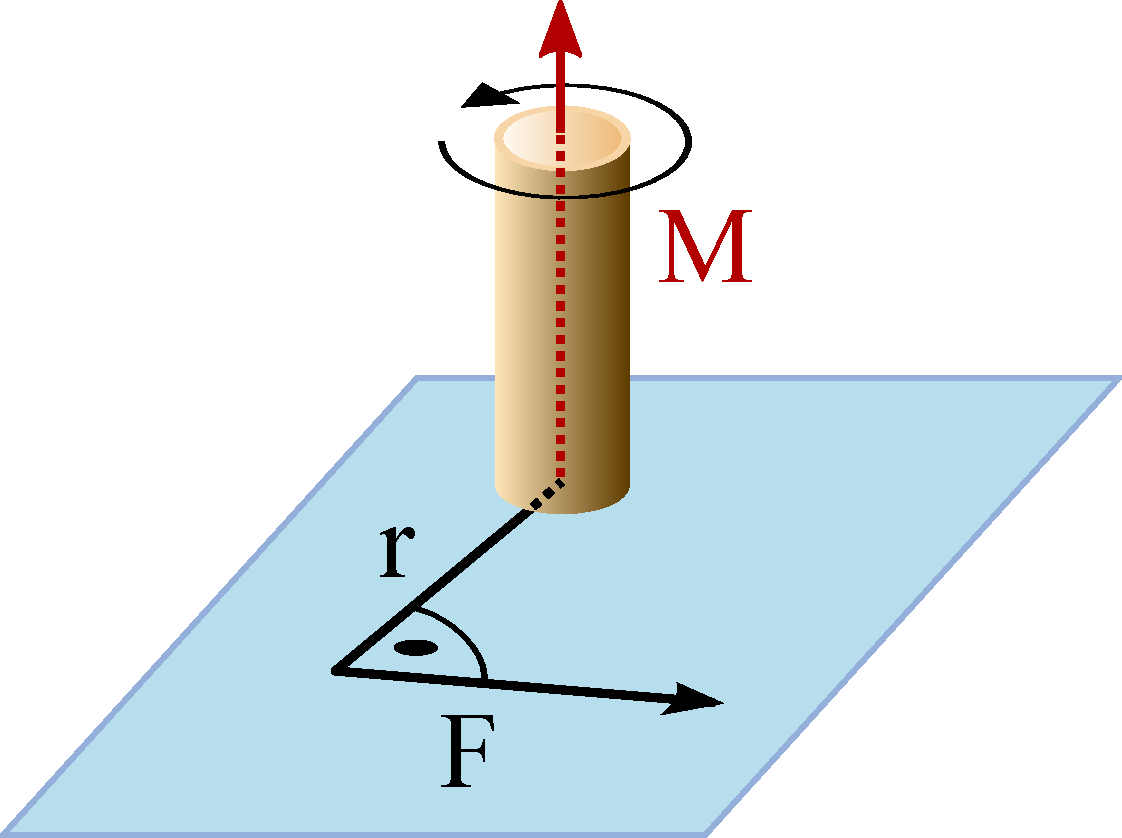
\includegraphics[width = 4cm ]{images/drehmoment}\\
	Lichtgeschwindigkeit & $c = \dfrac{1}{\sqrt{\mu_0\varepsilon_0}}$
\end{tabularx}

\subsection{Differential-Rechnung}
$f'(x_0)=\lim\limits_{\Delta x\rightarrow 0}
\frac{f(x_0+\Delta)x-f(x_0)}{\Delta x}$\\
\begin{tabular}{llll}
	Kettenregel:	& $f\big(g(x)\big)$ &$=$ & $g'(x)\cdot f'\big(g(x)\big)$
	oder $\frac{d f(g(x))}{dx} = f'(g(x)) \cdot g'(x)$\\[0.1cm] Produktregel:	&
	$f(x)\cdot g(x)$ &$=$ & $f'(x)\cdot g(x) + f(x)\cdot g'(x)$\\[0.1cm] Quotientenregel:& $\frac{f(x)}{g(x)}$ &$=$ & $\frac{f'(x)g(x)-f(x)g'(x)}{g^2(x)}$\\
\end{tabular}


\subsection{Taylor Polynom}
$f(x_0+h)=f(x_0) + f'(x_0)h + \frac{f''(x_0)}{2}h^2 + \frac{f'''(x_0)}{3!}h^3 + \ldots + \frac{f^{(n)}(x_0)}{n!}h^n + R_n(x_0, h)$


\subsection{Integraltable}
\begin{center}	
	\begin{multicols}{2}
		
		\begin{equation}
			\int x^n \dx = \frac{1}{n+1}x^{n+1}, \hspace{1ex} n\neq-1
		\end{equation}
		
		\begin{equation}
			\int \frac{1}{x}\dx = \ln |x|
		\end{equation}
		
		\begin{equation}
			\int u \hspace{2pt} \dd{v} = uv - \int v du
		\end{equation}
		
		
		
		\begin{equation}
			\int e^x \dx = e^x 
		\end{equation}
		
		\begin{equation}
			\int a^x \dx = \frac{1}{\ln a} a^x
		\end{equation}
		
		\begin{equation}
			\int \ln x \dx = x \ln x - x
		\end{equation}
		
		
		\begin{equation}
			\int \sin x \dx = -\cos x
		\end{equation}
		
		\begin{equation}
			\int \cos x \dx = \sin x
		\end{equation}
		
		\begin{equation}
			\int \tan x \dx = \ln |\sec x| 
		\end{equation}
		
		\begin{equation}
			\int \sec x \dx = \ln |\sec x + \tan x|
		\end{equation}
		
		\begin{equation}
			\int \sec^2 x \dx = \tan x
		\end{equation}
		
		\begin{equation}
			\int \sec x \tan x \dx = \sec x
		\end{equation}
		
		\begin{equation}
			\int \frac{a}{a^2+x^2}\dx = \tan^{-1}\frac{x}{a}
		\end{equation}
		
		\begin{equation}
			\int \frac{a}{a^2-x^2}\dx = \frac{1}{2}\ln\left|\frac{x+a}{x-a}\right|
		\end{equation}
		
		\begin{equation}
			\int \frac{1}{\sqrt{a^2-x^2}} \dx = \sin^{-1} \frac{x}{a}
		\end{equation}
		
		\begin{equation}
			\int \frac{a}{x \sqrt{x^2-a^2}} \dx = \sec^{-1} \frac{x}{a}
		\end{equation}
		
		\begin{align}
			\int \frac{1}{\sqrt{x^2-a^2}} \dx &= \cosh^{-1} \frac{x}{a} \\&= \nonumber \ln (x+\sqrt{x^2-a^2})
		\end{align}
		
		\begin{align}
			\int \frac{1}{\sqrt{x^2+a^2}} \dx &= \sinh^{-1} \frac{x}{a} \\&=\nonumber \ln (x+\sqrt{x^2+a^2})
		\end{align}
		
	\end{multicols}
\end{center}		

